\section{Аналитический обзор программных продуктов, литературных источников}

\subsection{Основные понятия и определения в областа навигации мобильных систем } 

Автономная навигация мобильных систем означает, что робот перемещается в
окружающем пространстве, избегает препятствий и достигает поставленных целей.
Для этого необходимо знать позицию робота, карту окружающего пространства,
спланировать и выполнить спланированный маршрут.

В автономной навигации можно выделить 4 класса задач:
\begin{itemize}
	\item локализация -- определение позиции робота;
	\item картирование -- построение карты;
	\item планирование траектории -- построение траектории с текущей в целевую
		позицию;
	\item следование траектории -- отправка команд на шасси которые
		осуществляют перемещение следуюя траектории.
\end{itemize}

\subsubsection{Локализация}
Локализация -- есть мобильный робот, известна карта окружающего пространста но
неизвестна его позиция. С помощью информации с сенсоров необходимо определить
позицию в которой он находится.

\subsubsection{Картирование}
Картирование -- есть позиция робота и показания с сенсоров, необходимо
построить карту окружающего его пространства.

\subsubsection{Планирование траектории}
Планирование траектории - известна карта окружающего пространства, известна
изначальная позиция робота и известна конечная позиция. Необходимо проложить
траекторию от начально до конечной позиции избегая препятствий и учитывая
габариты и кинематические свойства робота.

\subsubsection{Следование траектории}
Следование траектории - известна карта окружающего пространства, известна
текущая позиция робота и траектория. Необходимо сформировать команды управления
для следования роботом данной траектории.

\subsubsection{SLAM}
Когда задачи локализации и картирования возникают одновременно, что нет точной
позиции робота и нет карты местности, то возникает проблема что необходимо
решать задачу одновременной локализации и картирования. Данную задачу
невозможно решить раздельно с помощью локализации и картирования, из-за того
что для построения карты необходимо знать текущую позицию, а для определения
текущей позиции необходима карта. Для её решение применяется метод SLAM (англ.
simultaneous localization and mapping -- одновременная локализация и
картирование).

Метод одновременной навигации и построения карты связывает два независимых
процесса в непрерывный цикл вычислений, где результаты вычисления одного
процесса участвуют в вычислениях другого процесса.

\subsection{Обзор аналогов}
% - В основном всё закрытое и мало чего в открытом доступе.
% - Есть ROS который де-факто стандарт и его пакеты.
% - Проблема ROS в его изначально настройке и развёртке
% 	- Разворачивать можно только на специфичной версии убунты
% 	- Своя система сборки
% 	- Из-за особенностей архитектуры, пакеты общаются между собой через
% 	  систему сообщений, пересылая в некоторых моментах огромные объёмы
% 	  данных.

В программировании роботов активно используются фреймворки для межпроцесного
взаимодействия между отдельными модулями\footnote{Под модулями подразумеваются
отдельные программы, являющиеся компонентами системы, исполняющиеся в отдельных
процессах операционной системы, или даже на отдельных компьютерах.}. Примером
таких фреймворков служат \ros{} и YARP.

Это позволяет разрабатывать ПО с использованием разных языков программирования,
осуществлять переиспользование отдельных модулей, анализировать и записывать
потоки сообщений, настраивать маршрутизацию сообщений.

\subsection{Robot operating system}
\ros{} является де-факто стандартным фреймворком для программного обеспечения
роботизированных систем \cite{albonico2023software}. Статья
\selectlanguage{english}
"Software engineering research on the Robot Operating System: A systematic
mapping study"
\selectlanguage{russian}
\cite{quigley2009ros} процитирована более \num{13000} раз.

\ros{} предлагает использовать распределённые программы (также известные как
ноды), что позволяет разрабатывать исполняемые файлы индивидуально, и свободно
сочетать их во время исполнения. Эти процессы могут быть объединены в пакеты и
стэки, которыми можно легко делится и распространять.
\ros{} поддерживает единую систему кодовых репозиторириев которые
позволяют сотрудничеству быть распределённым.

Отличительные характеристики \ros{} можно кратко сформулировать следующим образом
 \cite{quigley2009ros}:
\begin{itemize}
	\item общение модулей происходит в одноранговой сети;
	\item использование готовых иструментов;
	\item возможность использования различных языков программирования;
	% \item тонкий; % Тут было thin, как thin перевести я не знаю, типо не
		% явлется штукой с огромным списком фич, а лишь прослойкой для общения
		% TODO
	\item свободный и открытый исходный код.
\end{itemize}

На данный момент существует две версии \ros{}: \ros{}1 и \rosTwo{}. Первый
официальный релиз \ros{} (под кодовым названием ROS Box Turtler) состоялся 2
марта 2010 года. Первый официальный релиз \rosTwo{} состоялся 8 декабря 2017
года. \rosTwo{} это более расширенная версия \ros{}, спроектированная чтобы
устранить недостатки \ros{} 1, такие как: масштабируемость, производительность и
кросс-платформенная совместимость. Поддержка \ros{} 1 заканчивается 31 мая 2025
года. 
% Далее в дипломной записке при упоминании \ros{} идёт речь о \rosTwo{}.
% \todo{А так можно?}


\subsubsection{Nav2}
В экосистеме \ros{} есть готовый фреймворк для навигации -- Nav2
\cite{macenski2020marathon2}. Nav2 - это новая версия фреймворка
разработанная для \rosTwo{}, в котором используются те же технологии, что и в
автономных транспортных средствах, уменьшенные, оптимизированные и
переработанные для мобильной робототехники. Этот проект позволяет мобильным
роботам перемещаться по сложным средам для выполнения заданных пользователем
прикладных задач. Nav2 - это высококачественный навигационный фреймворк
промышленного уровня, которому доверяют более 100 компаний по всему миру.

\begin{figure}[h]
\centering
	\fbox{
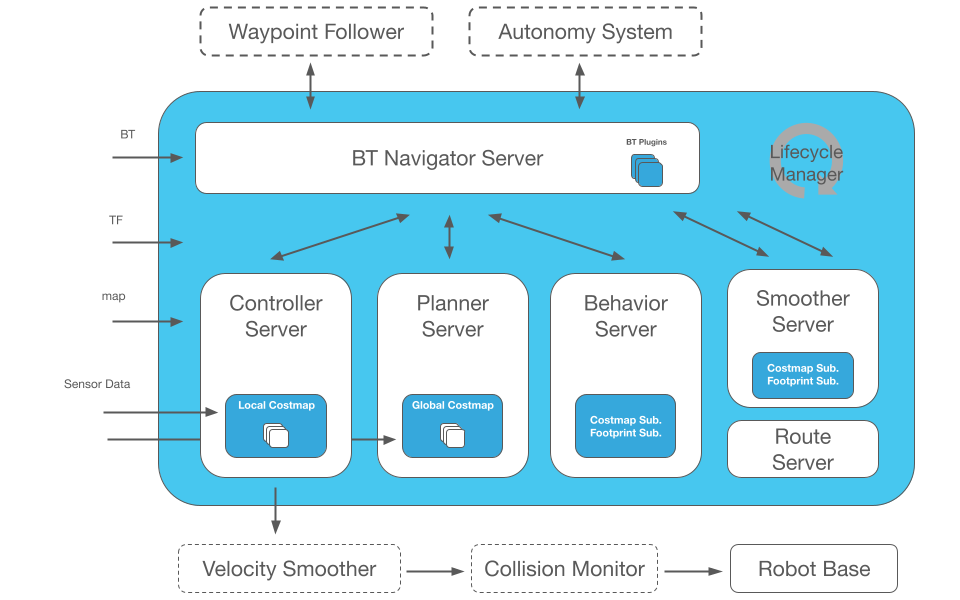
\includegraphics[width=14cm]{nav2_architecture}
}
\caption{Архитектура стэка Nav2}
\end{figure}

В Nav2 есть инструменты для:
\begin{itemize}
	\item загрузки и сохранения карт;
	\item локализации робота по предоставленной карте;
	\item планирования пути через окружающую среду;
	\item управления роботом, чтобы он следовал по маршруту и динамически
		корректировался, чтобы избежать столкновений;
	\item сглаживания маршрутов, чтобы сделать их более плавными;
	\item преобразование данных датчиков в модель окружающего мира;
	\item построение сложных и настраиваемых моделей поведения роботов с
		помощью деревьев поведения;
	\item выполнение заранее определенных действий в случае сбоя, вмешательства
		человека или других ситуаций;
	\item выполнение последовательных маршрутных точек, составляющих миссию;
	\item управление жизненным циклом программы и сторожевым таймером для
		серверов;
	\item мониторинг необработанных данных датчиков на предмет неминуемого
		столкновения или опасной ситуации;
\end{itemize}

\subsection{Анализ пакетов \ros{} решающих задачу одновременной локализации и
картирования}
\label{sec:ros_analysys}

Алгоритмы SLAM можно разделить на две группы: более ранние алгоритмы,
использующие подходы, основанные на фильтрах Байеса, и более новые методы,
основанные на графах. Значимые реализации на основе фильтров, доступные в виде
пакетов \ros{}: GMapping и HectorSLAM. Cartographer и KartoSLAM являются
основными доступными реализациями на основе графов \cite{macenski2021slam}.

Рассмотрим пакеты ros{}, такие как: SLAM Toolbox и GMapping:
\begin{itemize}
	\item SLAM Toolbox -- использует подход оптимизации
		графов.
	\item GMapping \cite{grisetti2005improving} -- использует Rao–Blackwellized
		Particle Filter (Фильтр частиц с использование теоремы Рао -- Блэквелла --
		Колмогорова )
\end{itemize}

% SLAM Toolbox 
% В SLAM Toolbox есть возможность делать почти всё, что есть в любой другой
% платной и бесплатной библиотеке SLAM. Это включает в себя:
В SLAM Toolbox реализованы многие функции которые необходимы для навигации и
постройки карт
\begin{itemize}
	\item точечный 2D SLAM для мобильных роботов, с экспортом карт;
	\item продолжение уточнения карты после остановки, перестройка карты или
		продолжение построения карты из сохраненного файла позиций в любое
		время;
	\item пожизненное картирование -- продолжение построение карты  в течении
		всей работы ПО, одновременно удаляя лишнюю информацию из новых снимков
		лидара.
	\item режим локализации на основе, построенный на основе графа позиций.
		Возможность запуска режима локализации без предварительной карты для
		режима «лидарной одометрии» с локальным замыканием циклов;
	\item синхронный и асинхронный режимы работы;
	\item оптимизационные решатели на основе плагинов с новым оптимизированным
		плагином на основе Google Ceres;
	\item плагин RVIZ для взаимодействия с инструментами;
	\item инструменты манипулирования графами в RVIZ для манипулирования узлами
		и связями графа во время отображения;
	\item сериализация карт и хранение данных без потерь.
\end{itemize}

\begin{figure}[h]
\centering
	\fbox{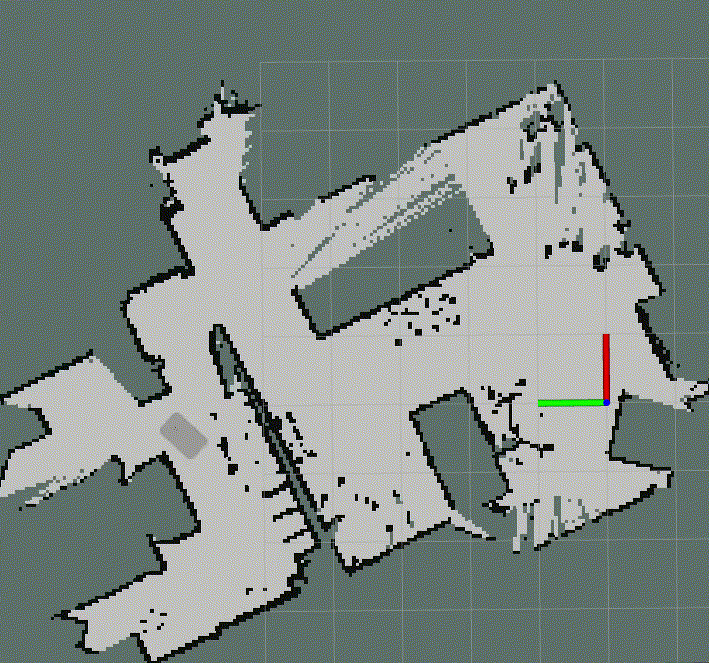
\includegraphics[width=7cm]{slam_toolbox_example}
\centering
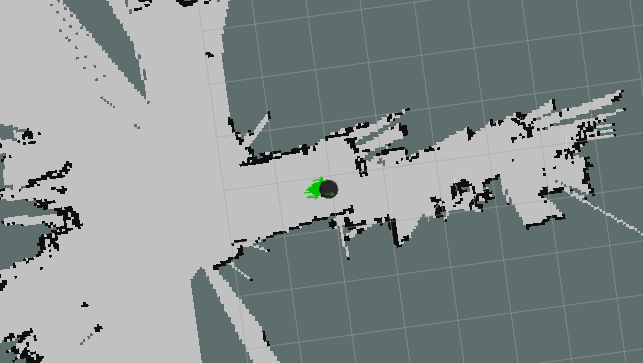
\includegraphics[width=7cm]{gmapping_example}
	}
	\caption{Пример построения карты используя SLAM Toolbox (слева) и GMapping
	(справа).}
	\label{ris:map_example}
\end{figure}

В то время как пакет GMapping предлагает обёртку над алгоритмом,
описанным в статье \cite{grisetti2005improving}, не включая дополнительный
функционал который предоставляется SLAM Toolbox, предоставляя лишь возможность настройки параметров алгоритма и получения построенной карты.




\subsection{Yet Another Robot Platform}
Yet Another Robot Platform (YARP) \cite{metta2006yarp} -- это фреймворк который
преследует цели, очень схожие с \ros{}. YARP поддерживает построение системы
управления роботом как набор программ общающимся в одноранговой сети используя
различные каналы связи, что по своей сути не отличается от целей ros{}. YARP
менее популярен, используется для более специализированных систем и не имеет
отличительных преимуществ, поэтому далее его не рассматриваем.


\subsection{Формирование требований к проектируемому программному средству}

% \todo{Формирование требований}
%
% Исходя из результата анализа существующих аналогов, можно выделить следующие недостатки:

% \begin{itemize}
% 	\item \todo{Недостаток 1}
% \end{itemize}

Исходя из этого, целью дипломного проектирования является разработка
программного средства, способного устранить вышеперечисленные недостатки, а
также реализовать необходимый набор функций характерный для программных средств
в этой области.

Для достижения поставленных целей следует решить следующие задачи: 
\begin{itemize}
	\item определить требования  к  разрабатываемому  программному  средству  и 
	составление спецификации, включающей их; 
	\item осуществить выбор  технологии  и  языка  программирования  для
		реализации программного средства; 
	\item провести проектирование архитектуры программного средства; 
	\item разработка алгоритмов для метода SLAM; 
	\item разработка алгоритмов для оценки местоположения; 
	\item разработка алгоритмов для поиска маршрута; 
	\item разработка алгоритмов для выполнения маршрута; 
	\item программирование и тестирование отдельных программных модулей; 
	\item тестирование готового программного средств.
\end{itemize}

% \todo{Набор функций}

% Для достижения поставленной цели необходимо решить следующие недостатки:
%
% % - Уменьшить потребление памяти
% % - Моментальное обновление карты
% % - Single binary executable
% % - speed of execution
%
% \begin{itemize}
% 	\item \todo{Недостаток}
% \end{itemize}
